\lecture{Задача локализации точки}{Ефим Перевалов}

Пусть дан некоторый многоугольник $M$ и точка $p$. Требуется определить, лежит ли $p$ внутри $M$.

\subsection{Многоугольник выпуклый}

\

Если многоугольник $M$ выпуклый, то можно пустить луч из точки $p$ и посчитать количество пересечений.

\hspace{1cm} 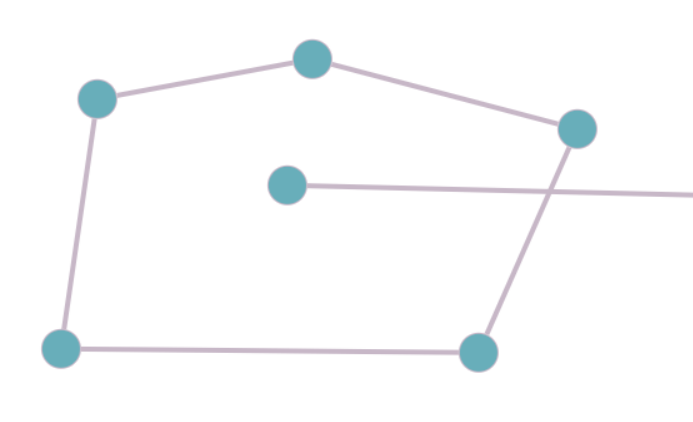
\includegraphics[height=6cm, width=10cm]{vipukli.png}

\

Возможны три случая:
\begin{enumerate}
    \item Луч не пересекает ни одну из сторон -- тогда $p$ не лежит в $M$
    \item Луч пересекает одну сторону -- $p$ находится внутри $M$
    \item луч пересекает две стороны -- $p$ не лежит в $M$
\end{enumerate}

\

Асимптотическая оценка $O(n \cdot log(n))$. Быстрее чем за линию не получится, так как, как минимум, нужно считать все вершины.

\

Поиск стороны будет осуществляться с помощью банарного  поиска, поэтому время выполнения оценивается как $O(log(n))$

\subsection{Многоугольник невыпуклый}

\

Если многоугольник $M$ невыпуклый, то можно пустить луч из точки $p$ и если количество пересечений не четное, то точка находится внутри.

\hspace{1cm} 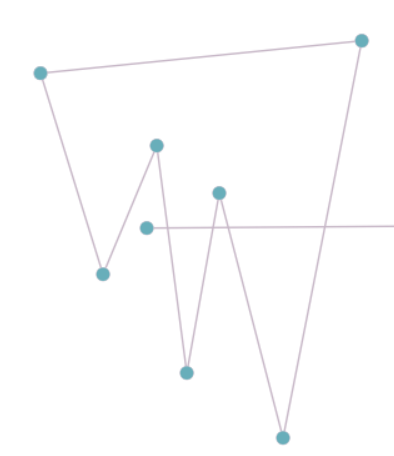
\includegraphics[height=6cm, width=10cm]{nevipukli.png}

\

Бинарный поиск в данном случае не поможет, так как слишком много пересечений. Можно использовать алгоритм, который будет делить многоугольник на слои. Проведем прямые по линии абсцисс в вершинах.

\hspace{1cm} 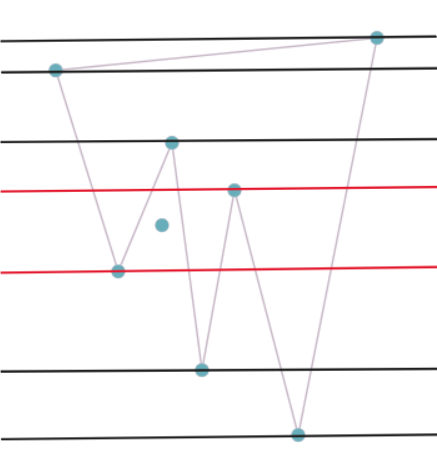
\includegraphics[height=4cm, width=10cm]{sloi.png}

\

Берем слой с точкой и ищем где она находится: внутри или снаружи.

\hspace{1cm} 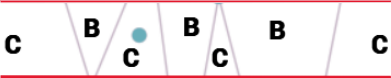
\includegraphics[height=1cm, width=9cm]{C_B.png}

\

Можно заметить, что для $k$ точек будет $k$ отрезков, поэтому для поиска точки можно использовать бинарный поиск. Тем не менее обработка выделения слоев и указания с и в в слоях занимает много времени. Поэтому предобработка работает за $O(n^2)$, а поиск за $O(log(n))$.

Памяти потребуется $O(n^2)$ так как выделение слоев происходит за $O(n)$ и указание позиций в слоях также $O(n)$.

\

Сделать быстрее чем сортировка не получится, но можно использовать оптимизации, использующиеся у сортировок. Например преобработку можно распараллелить или воспользоваться концепцией разделяй и властвуй, но не в классическом виде.

Строим выпуклую оболочку триангулируя всю область

Количество треугольников после триангуляции будет равно количеству вершин - 2.

Затем эти треугольники можно захешировать.

Оценка таже, что и в способе со слоями, но сложнее считать и проще параллелить.

\

\subsection{Алгоритм Кирк Патрика}

\

Пусть у нас есть некоторая $N$-вершинная триангуляция $G$ многоугольника $P$. Поместим её в объемлющий треугольник (рис. \ref{triang}).
Построим последовательность триангуляций $S_1, ..., S_{h(N)}$, $S_1 = G$, где $S_i$ получается из $S_{i - 1}$ следующим образом:
\begin{enumerate}
    \item Удалим некоторое количество неграничных и попарно-несмежных друг с другом вершин и инцидентные им ребра.
    \item Построим триангуляцию получившегося многоугольника.
\end{enumerate}
Тогда $S_{h(N)}$ --- это объемлющий треугольник.

Теперь построим структуру данных для поиска. Пронумеруем треугольники в каждой триангуляции и обозначим их $R_k$.
Будем говорить, что треугольник $R_k$ принадлежит триангуляции $S_k$, если он был получен во время построения $k$-ой триангуляции.
Структура $T$ будет представлять из себя корневое дерево, где объемлющий треугольник --- это корень, а треугольники из $S_1$ --- листья.
Из треугольника $R_j$ будет вести ребро в треугольник $R_j$ если при построении $S_i$ из $S_{i - 1}$:
\begin{enumerate}
    \item $R_j$ удаляется из $S_{i - 1}$
    \item $R_k$ создается в $S_i$
    \item $R_k \cap R_j = \varnothing$.
\end{enumerate}

Поиск в структуре $T$ будет осуществляться следующим образом:
\begin{itemize}
    \item Точка $z$, очевидно, принадлежит объемлющему треугольнику
    \item Проверим детей на принадлежность им точки $z$
    \item Как только нашли потомка, которому принадлежит $z$, переходим в него и снова переходим к шагу 2.
\end{itemize}
Таким образом, выполняется последовательная локализация в триангуляциях $S_1, S_2, ..., S_{h(N)}$ (рис. \ref{bild_triang}).

\begin{figure}[h]
    \centering
    \def\svgwidth{0.3\columnwidth}
    \input{./lecture02/triangulation.pdf_tex}
    \caption{Триангуляция в объемлющем треугольнике}
    \label {triang}
\end{figure}

\begin{figure}[h]
    \centering
    \def\svgwidth{0.8\columnwidth}
    \input{./lecture02/triangulation_build.pdf_tex}
    \caption{Последовательность триангуляций}
    \label {bild_triang}
\end{figure}

\paragraph{Выбор вершин}
Эффективность алгоритма Киркпатрика напрямую зависит от выбора вершин для удаления в шаге 1.
Предположим, что можно выбрать множество удаляемых вершин так, что:
\begin{enumerate}
    \item $N_i = a_i N_{i - 1}$, где $a_i \leqslant a < 1$ и $N_i$ --- число вершин в $S_i$
    \item Каждый треугольник $R_i \in S_i$ пересекается не более чем с $H$ треугольниками из $S_{i - 1}$, и наоборот.
\end{enumerate}
Тогда $h(N) \leqslant \log_{1 / a} N = O(\log N)$, а также $T$ занимает $O(N)$ памяти.

Если удалять несмежные вершины со степенью меньше $12$, то свойства, описанные выше, выполняются.
